\section{Border ASes and Chokepoint Potential}

\Ben[inline]{Include a little paragraph here about what this section describes}.

\begin{figure}
	\centering
	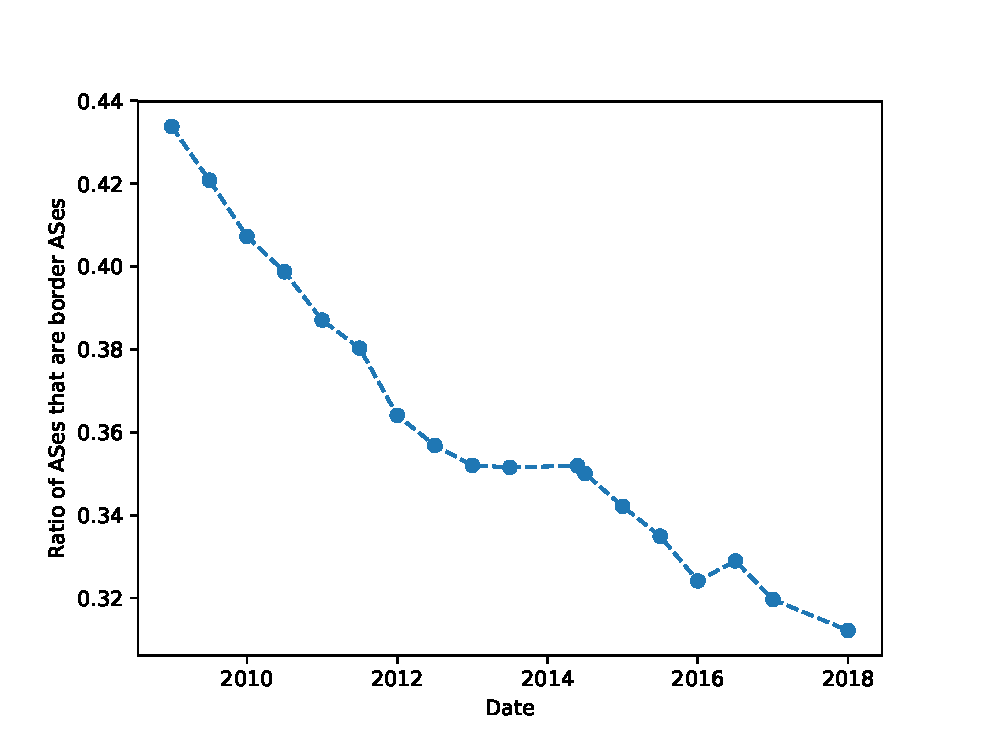
\includegraphics[width=\linewidth]{bnodes}
	\caption{The ratio of ASes that are border ASes plotted over several years.}\label{fig:bnodes}
\end{figure}

\begin{figure}
	\centering
	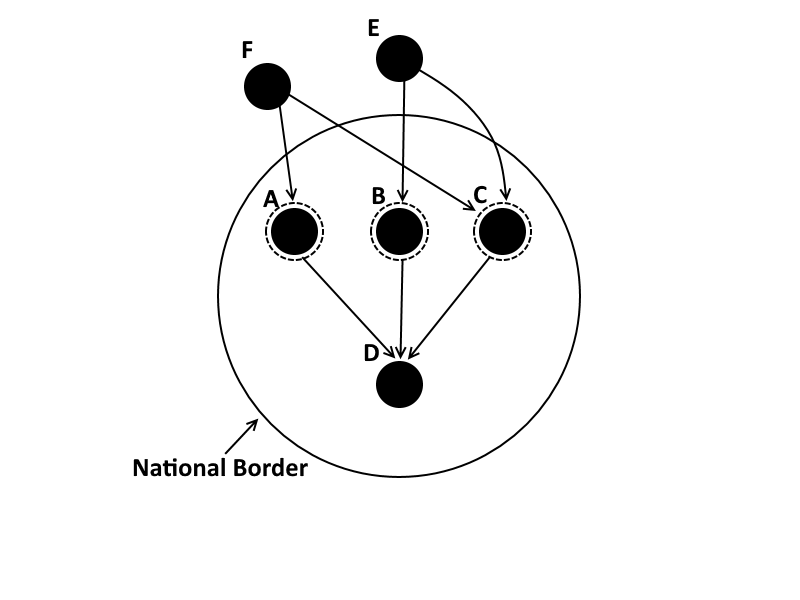
\includegraphics[width=\linewidth]{chokepoint}
	\caption{Chokepoint potential example. ASes A,B, and C are all border ASes. 
						AS D is an internal AS. ASes E and F are both external ASes.
						The out-to-in chokepoint potentials of A,B, and C are 0.25, 0.25, and 0.5 respectively.}\label{fig:chokepoint}
\end{figure}

\subsection{Border Nodes}

Border ASes are ASes that lie adjacent from an AS registered to a different
country along a routing path. More formally, we define $g(\cdot)$ as the
mapping from ASes to the country of registration, and say an AS $a_u$ is a border
AS if $g(a_u) \neq g(a_v)$, where $a_v$ is a neighboring AS.  Because of their
position along national border, these ASes, can act as convenient locations for
national governments to control information flow into or out of a country. This
is especially true if a large number of BGP paths traverse a small number of
border ASes. Even as countries expand their Internet infrastructure, they may
be concentrating traffic that crosses national borders to a small number of
governmentally controlled ASes.  Evidence for this can be seen in the ratio of
the number of border ASes of a country to all ASes in that country.
%hints toward the abillity of that nation to intercept information flows across
%their borders.
\figurename \ref{fig:bnodes} shows that globally the number of border ASes has
grown at a slower rate than the number of non-border ASes.
%over time so that the ratio of border ASes to ASes has almost continuously
%decreased. 
It would seem that this fact reflects an ever increasing capability for nations
to intercept AS-level paths.  However, an important consideration is not only
how many border nodes exist, but also how often each is utilized in BGP
routing. Because AS-level paths are generated by distributed BGP routing tables
and the local preferences of AS administrators, a better way to understand the
potential for bottlenecks on border ASes is to investigate the number of BGP
generated paths that pass through each AS. We propose an intuitive measure of
AS bottlenecks called \emph{chokepoint potential}. Surveillance and censorship
generally occurs at a national level so we further define an aggregate measure
for nations, which we call \emph{national chokepoint potential}.

% % Why Border ASes?
% In order to identify AS chokepoints and compare nations, we need a measure that can be calculated from the many paths between
% ASes. First, we decided to use a measure that is evaluated only on border ASes, or ASes that lie one hop from an AS belonging to another nation. 
% The evolution of AS relationships and national boundaries on the AS graph hints that border ASes are an important feature in regards to the flow
% of information. Consider that while the number of ASes globally has continued to grow rapidly, the number of border ASes has grown more slowly.
% This result is depicted in figure \ref{fig:bnodes}. Additionally, while internal chokepoints may intercept many paths, those paths are required
% to have entered through a border AS (in the case of out-to-in paths) or exit through a border AS (for in-to-out paths). This focus on border ASes has
% the added benefit of making calculations more efficient.

\subsection{Chokepoint Potential}

We define a BGP path of length $n$ from source AS $a_0$ to destination AS $a_n$
as a sequence $p_{1\rightsquigarrow n} = \{a_i : i \in [1,n]\}$.  We define a
\textit{routing tree} to be a tree rooted at a single destination AS and
composed of every acceptable BGP path from the various source ASes that can
reach the destination AS.\Ben[inline]{Is this always a tree? Seems like it
could be a DAG sometimes (especially if random choices are made). Also do we
need to define routing trees if we only really work on the path}  The
chokepoint potential of a border AS is the ratio of paths intercepted by that
border AS to the number of paths intercepted by all border ASes belonging to
the same nation. Formally, for a country $c$, let $P = \{p_{i \rightsquigarrow
j} : g(a_i)=c \text{ and } g(a_j)\neq c\} $, i.e.\ the set of all path
originating in $c$ and ending in outside $c$. Then the chokepoint potential,
$cp(\cdot)$, of a border AS $a_u$ with $g(a_u) = c$ is

\begin{equation}
  \label{eq:chokepoint}
  cp(a_u) = \frac{|\{p: p \in P \text{ and } a_u \in P\}|}{|P|}
\end{equation}

The above definition is specifically for capturing paths originating in country
$c$ and routing outside the country, which we will refer to as
\textit{outgoing} chokepoint potential or $cpo$. We can similarily define
\textit{incoming} chokepoint potential or $cpi$, by simply redefining $P$ as $\{p_{i
\rightsquigarrow j}: g(a_i) \neq c \text{ and } g(a_j) = c\}$. That is all
paths originating outside of $c$ but terminating in $c$ and recomputing
Equation~\ref{eq:chokepoint}. 

%For instance, take
%a border AS $b$, belonging to country $c$.  If $P_c$ is the set of paths in to
%or out of country $c$ and $B_p$ is the set of border ASes within path $p$, then
%the chokepoint potential of $b$, $CP(b)$ is defined formally in equation
%\ref{eqn:chokePointPotential}. 
%This is calculated seperately for in-to-out paths (those starting from a source
%in the country in question) and out-to-in paths.
The incoming chokepoint
potential for a nations is illustrated in \figurename
\ref{fig:chokepoint}.

\Ben[inline]{A couple of questions here. Why mess with incoming (out to in) and
outgoing (in to out) measures? Can we just define it as $\frac{|p_{in}| +
|p_{out}|}{|P_{in}| + |P_{out}|}$, that is the incoming and outgoing paths over
the total paths? Would this be that much different? Is there are an argument to
be made that out-to-in or in-to-out is a better? My guess is they are all
pretty correlated, I can check on that}.
% Formal Definition
%\begin{equation}\label{eqn:chokePointPotential}
%CP(b) = \frac{|\{p \in P_c \textrm{ s.t. } \{b\} \subseteq B_p\}|}{\sum_{p \in P_c}|B_p|}
%\end{equation}

Given a set of routing trees\Ben[inline]{paths?}, chokepoint potential is an intuitive way to
compare individual ASes. With this measure, the sum of the chokepoint potential
for all border ASes for a country is 1.0, as in, all of the border ASes
collectively control the flow of information over the nation's border. We
define the aggregate \emph{national chokepoint potential} as the number of
border ASes required to control a particular fraction $f$ of paths. Formally,
given a country,$c$, with a set of $k$ border ASes $\{a_1,a_2,\cdots,a_k\}$ with
$cp(a_i)>cp(a_j) \forall i<k$ (i.e.\ sorted in descending order), the
we find the smallest $j$ such that 

\begin{equation}
  \label{eq:nationalchokepoint}
  \sum_{i=1}^j cp(a_i) > f
\end{equation}

and define national chokepoint potential as $CP(c,f) = 1/j$. We use the
multiplicative inverse here to preserve a clearer semantic meaning i.e.\ higher
chokepoint potential implies more control over paths. The more border ASes
required, the more difficult it would likely be for that nation to perform
censorship or surveillance, as the government would have to restrict more ISPs,
place more filtering hardware, etc. 
%Thus, we can define another measure, with
%this one being a national measure. We define the \emph{national breakthrough
%potential} of a nation to be the minimum number of ASes required to intercept a
%selected percentage of AS-level paths. 
Previous work has used $f=0.90$ as a benchmark indicating strong control of information
\cite{throats}, so we use this percentage as well. When used here, however,
90\% path interception indicates a single nation intercepts 90\% of the paths
that either enter said nation (for the out-to-in case) or exit said nation (for
the in-to-out case). National breakthrough potential is calculated taking the
strongest ASes first, such that the measure reflects the smallest number of
border ASes needed to intercept the paths.\footnote{We note that a dual measure
could be defined as the fraction of paths controlled by $j$ ASes. Our results
are substantively the same for either definition.\Ben[inline]{Check to make
sure}}. 

We measure the absolute number of ASes required to control a specific
fraction rather than a percentage within a country because it makes for more
equitable comparisons between nations
Take for instance the United States, which has many more ASes than
most nations. If the United States and another nation both required the same
percentage of border ASes to intercept 90\% of paths, the similarity of these
nations would be misleading. Controlling the larger absolute number of ASes
would require significantly more resources.\Ben[inline]{we need to actually
pick another nation where this is true to make this example illustrative.} Our technique provides a comparison more likely to
reflect reality. 
%This measure is called a breakthrough potential because it
%indicates the number of border ASes that intercept a vast majority of paths,
%meaning that a country with high NBP would require controlling many border ASes
%to prevent a breakthrough, or an unfettered access of internal ASes to that
%country.
